%%%
% set up document type
%%%
\documentclass[12pt]{article}

%%%
% declare all packages
%%%
\usepackage[left=25mm, top=20mm, right=25mm, bottom=30mm,nohead,nofoot]{geometry} 

\usepackage[T2A]{fontenc}
\usepackage[utf8]{inputenc}
\usepackage[english, russian]{babel}

\usepackage{graphics, graphicx}

\usepackage{url}
\usepackage{hyperref}

\usepackage{amssymb,latexsym} 
\usepackage{MnSymbol}
\usepackage{mathrsfs}

\usepackage[nottoc,numbib]{tocbibind}
\usepackage{float}
\usepackage{listings}
\usepackage{multirow}
\usepackage{hhline}

\usepackage{color,colortbl}

%%%
% document settings
%%%
\setcounter{tocdepth}{4}
\graphicspath{ {./pic/} }

\renewcommand{\listoffigures}{\begingroup  % add number to list of graphics
\tocsection
\tocfile{\listfigurename}{lof}
\endgroup}
\renewcommand{\listoftables}{\begingroup  % add number to list of tables
\tocsection
\tocfile{\listtablename}{lot}
\endgroup}

%******************************************************************
%******************************************************************
\begin{document}

\begin{titlepage}
	\center
		Санкт-Петербургский Политехнический 
		университет Петра Великого
		Институт прикладной математики и механики
		\\ \textbf{Кафедра «Прикладная математика»}

	\vfill ~
	\textbf{
		\\ \large ЛАБОРАТОРНАЯ РАБОТА №4
	}
	\\	по дисциплине 
	\\	"Математическая статистика"

	\vfill ~

	Выполнил студент гр. \textbf{33631/1} \\
	\textbf{Лансков.Н.В.} \\ 

\vfill

{\large}	Санкт-Петербург
\\ 2019
\end{titlepage}

%%%
% Table of conetnts 
%%%

\tableofcontents 
\newpage
\listoffigures
\newpage
% \listoftables
% \newpage

%%%
% Text
%%%
\section{Постановка задачи}

Для, приведённых ниже, пяти распределений сгенерировать выборки объёмом $20,\; 60,\; 100,$ для каждой выборки построить эмпирические функции распределения и ядерные оценки плотности распределения на отрезке $[-4, 4].$

Распределения \cite{distr_formulas}:
\begin{enumerate}
\item Стандартное нормальное распределение
\item Стандартное распределение Коши
\item Распределение Лапласа с коэффициентом масштаба $\sqrt{2}$ и нулевым коэффициентом сдвига.
\item Равномерное распределение на отрезке $\left[-\sqrt{3}, \sqrt{3}\right]$
\item Распределение Пуассона со значением матожидания равным двум.
\end{enumerate}

\section{Теория}

Эмпирическая функция распределения \cite{emp}, построенная по выборке $X = \left(X_1,\ldots, X_n\right)$ есть случайная функция $F_n(y),$ определённая на $\mathbb{R}:$
\begin{equation}
F_n(y) = \sum\limits_{i=1}^n I\left(X_i < y\right) \;\;\text{где}\; I\left(X_i < y\right) = \begin{cases} 
1, & X_i < y\\
0, & \text{иначе}
\end{cases}\hfill\label{eqn:emp}
\end{equation}

$X = \left(X_1,\ldots, X_n\right)$ есть одномерная выборка одинаково распределённых элементов, с плотностью распределения $f.$

Ядерная оценка плотности \cite{art}:
\begin{equation}
    f_h(x) = \frac{1}{nh}\sum\limits_{i=1}^nK\left(\frac{x-x_i}{h}\right)\label{eqn:art}
\end{equation}
где $K$ является ядром, а $h>0$ является сглаживающим параметром, и называется шириной полосы.

В данной работе в качестве ядра была выбрана плотность вероятности стандартного нормального распределения \cite{link:pdf}:

\begin{equation}
    K(x) = \frac{1}{\sqrt{2\pi}}e^{-\frac{x^2}{2}}
\end{equation}

\section{Реализация}
Для генерации выборки был использован $Python\;3.7$: модуль $random$ библиотеки $numpy$ \cite{numpy} для генерации случайных чисел с различными распределениями. 

Обработка функций распределений была сделана с помощью модуля $scipy$ \cite{skp}.


\section{Результаты}

\subsection{Эмпирические функции распределения}
\begin{center}

\begin{figure}[H]
\caption{Эмпирическая функция для нормального стандартного распределения}
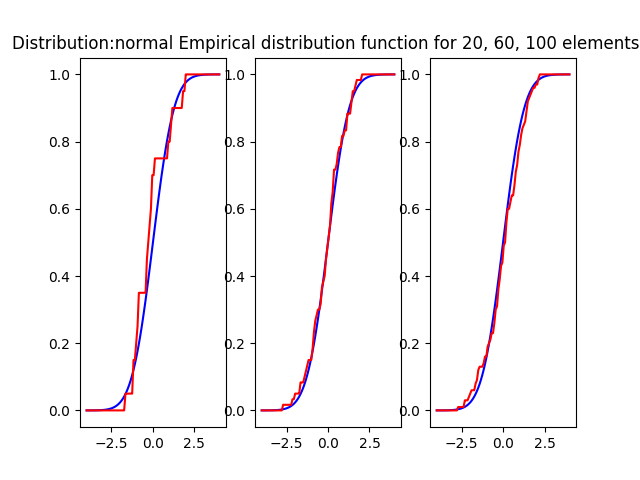
\includegraphics[width=\textwidth]{empiric/normal.png}
\end{figure}

\begin{figure}[H]
\caption{Эмпирическая функция для стандартного распределения Лапласа }
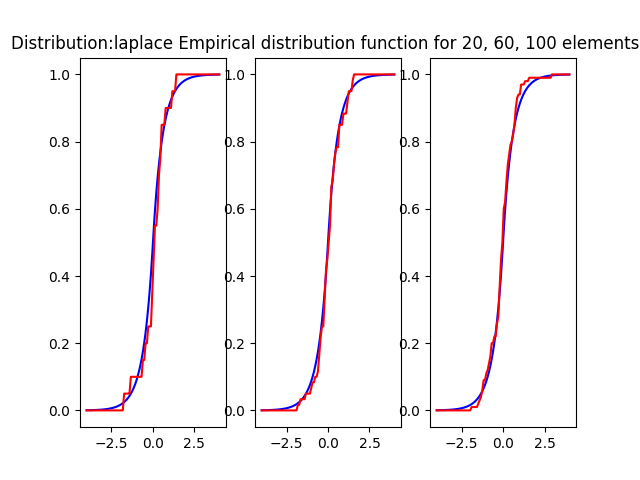
\includegraphics[width=\textwidth]{empiric/laplace.png} 
\end{figure}

\begin{figure}[H]
\caption{Эмпирическая функция для стандартного распределения Коши }
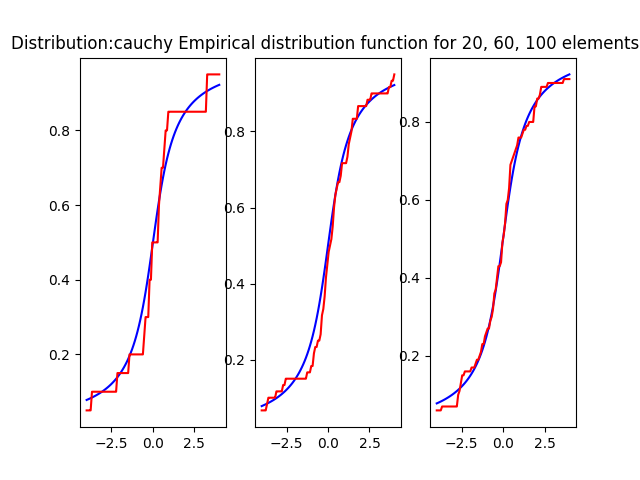
\includegraphics[width=\textwidth]{empiric/cauchy.png} 
\end{figure}

\begin{figure}[H]
\caption{Эмпирическая функция для распределения Пуассона }
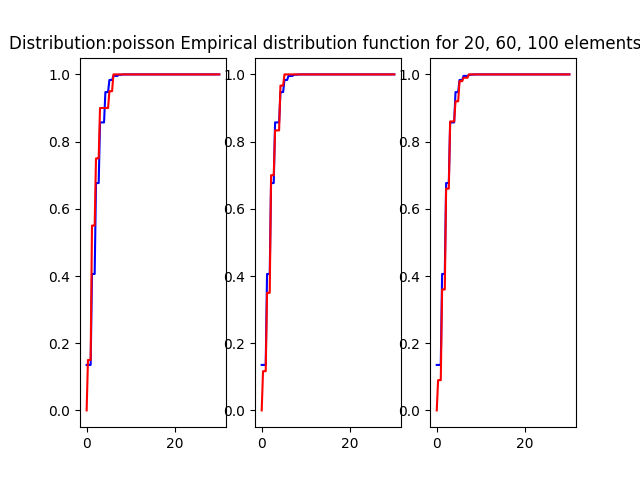
\includegraphics[width=\textwidth]{empiric/poisson.png} 
\end{figure}

\begin{figure}[H]
 \caption{Эмпирическая функция для равномерного распределения }
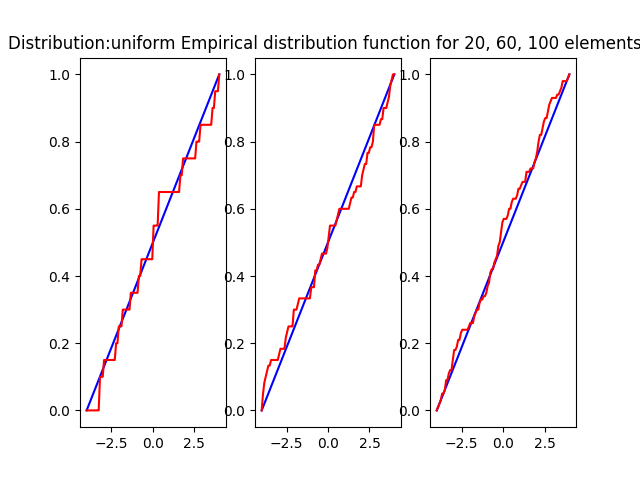
\includegraphics[width=\textwidth]{empiric/uniform.png}
\end{figure}
\end{center}
\subsection{Ядерные функции}

\begin{center}
    \begin{figure}[H]
 \caption{Ядерная функция плотности для нормального распределения, n = 20}
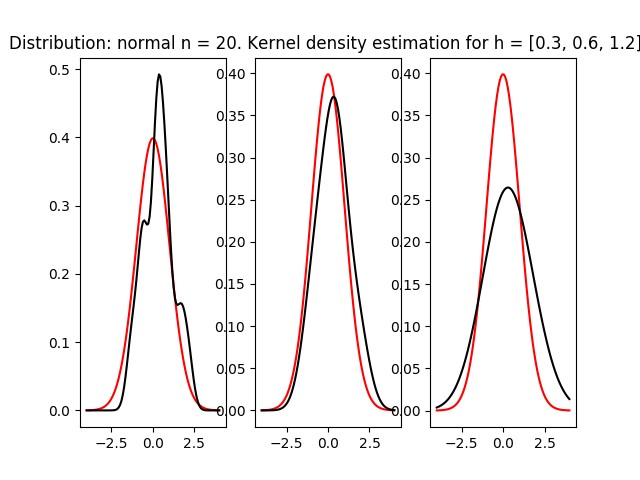
\includegraphics[width=\textwidth]{kernel/d_normal20.png}
\end{figure}
    \begin{figure}[H]
 \caption{Ядерная функция плотности для нормального распределения, n = 60}
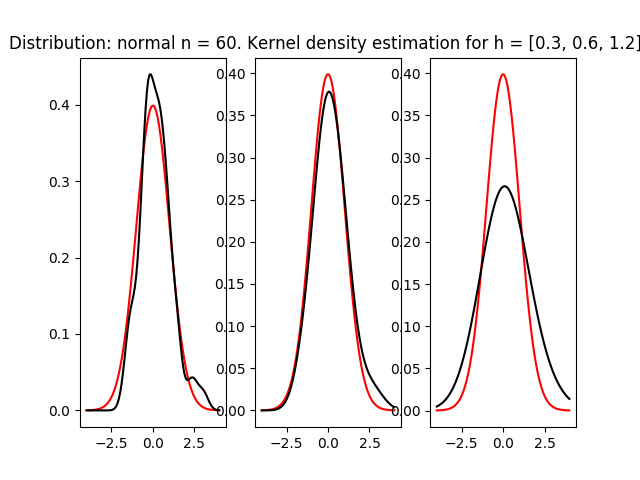
\includegraphics[width=\textwidth]{kernel/d_normal60.png}
\end{figure}
    \begin{figure}[H]
 \caption{Ядерная функция плотности для нормального распределения, n = 100}
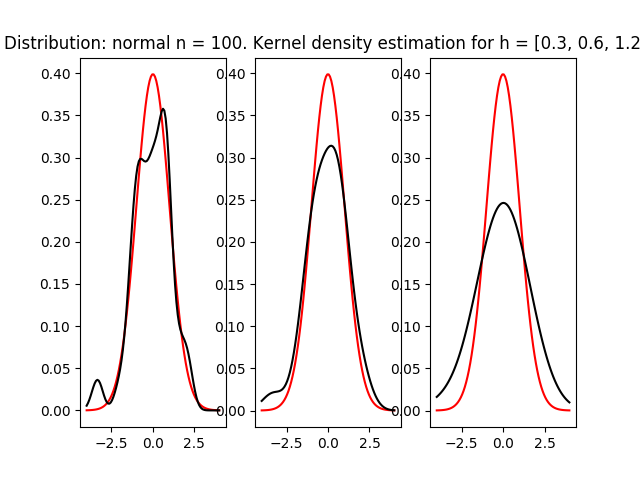
\includegraphics[width=\textwidth]{kernel/d_normal100.png}
\end{figure}

    \begin{figure}[H]
 \caption{Ядерная функция плотности для распределения Лапласа, n = 20}
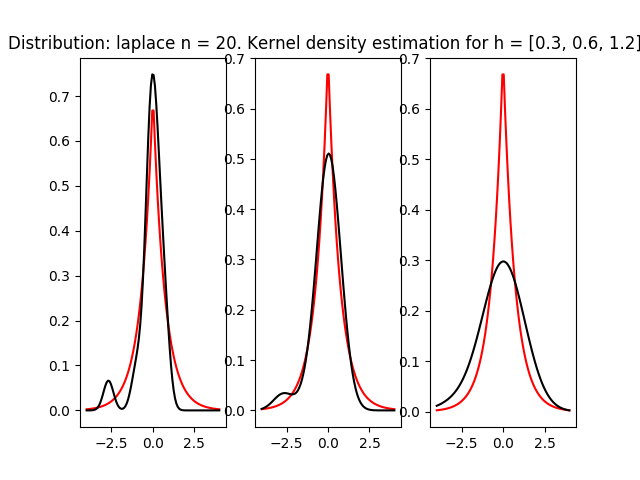
\includegraphics[width=\textwidth]{kernel/d_laplace20.png}
\end{figure}
    \begin{figure}[H]
 \caption{Ядерная функция плотности для распределения Лапласа, n = 60}
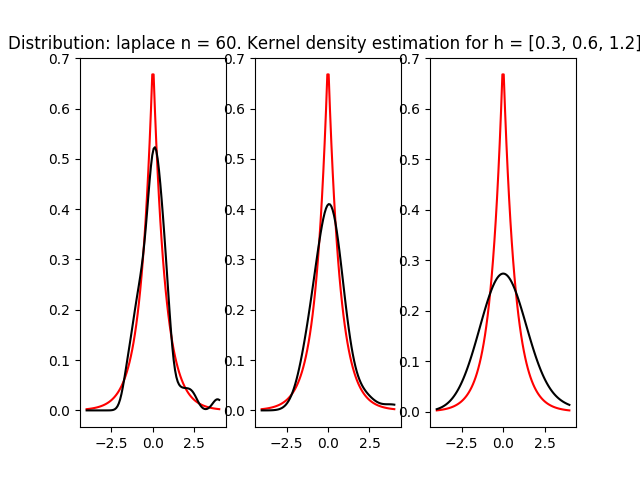
\includegraphics[width=\textwidth]{kernel/d_laplace60.png}
\end{figure}
    \begin{figure}[H]
 \caption{Ядерная функция плотности для распределения Лапласа, n = 100}
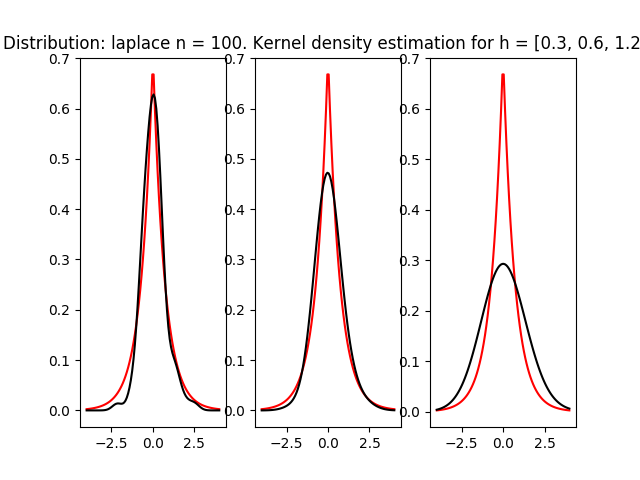
\includegraphics[width=\textwidth]{kernel/d_laplace100.png}
\end{figure}

    \begin{figure}[H]
 \caption{Ядерная функция плотности для распределения Коши, n = 20}
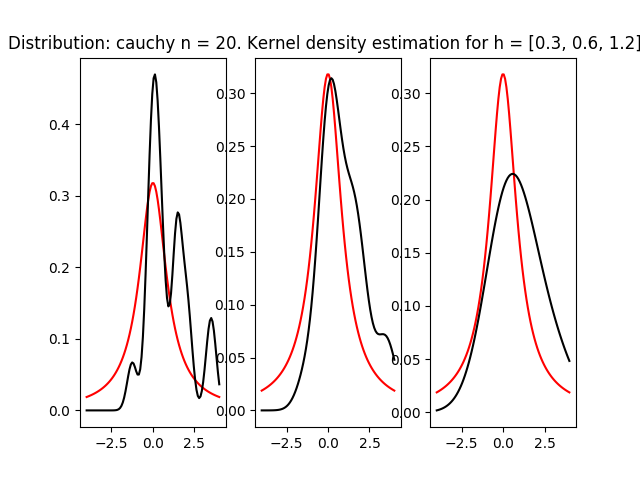
\includegraphics[width=\textwidth]{kernel/d_cauchy20.png}
\end{figure}
    \begin{figure}[H]
 \caption{Ядерная функция плотности для распределения Коши, n = 60}
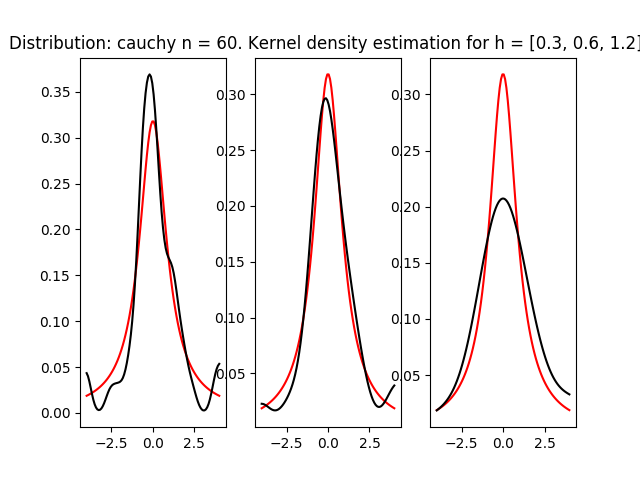
\includegraphics[width=\textwidth]{kernel/d_cauchy60.png}
\end{figure}
    \begin{figure}[H]
 \caption{Ядерная функция плотности для распределения Коши, n = 100}
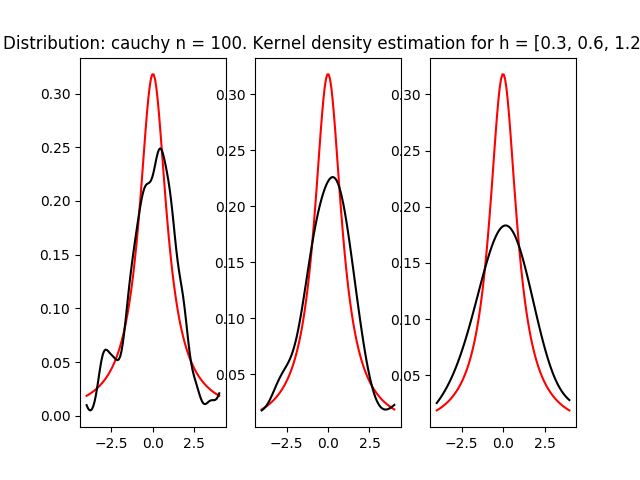
\includegraphics[width=\textwidth]{kernel/d_cauchy100.png}
\end{figure}

    \begin{figure}[H]
 \caption{Ядерная функция плотности для распределения Пуассона, n = 20}
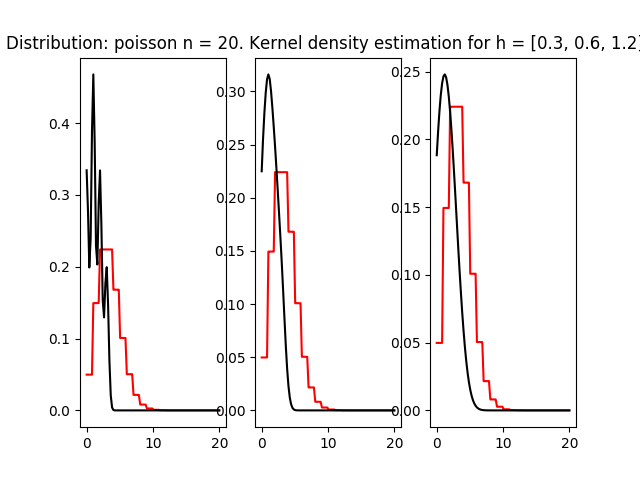
\includegraphics[width=\textwidth]{kernel/d_poisson20.png}
\end{figure}
    \begin{figure}[H]
 \caption{Ядерная функция плотности для распределения Пуассона, n = 60}
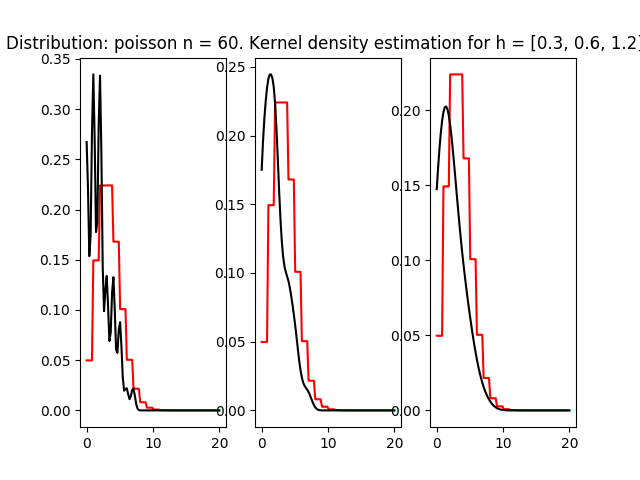
\includegraphics[width=\textwidth]{kernel/d_poisson60.png}
\end{figure}
    \begin{figure}[H]
 \caption{Ядерная функция плотности для распределения Пуассона, n = 100}
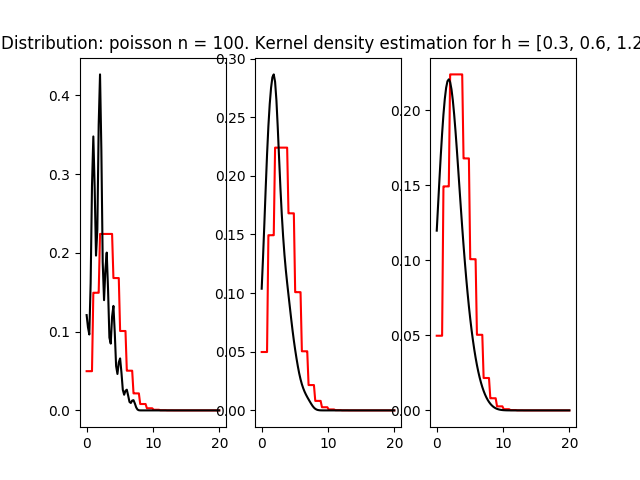
\includegraphics[width=\textwidth]{kernel/d_poisson100.png}
\end{figure}

    \begin{figure}[H]
 \caption{Ядерная функция плотности для равномерного распределения, n = 20}
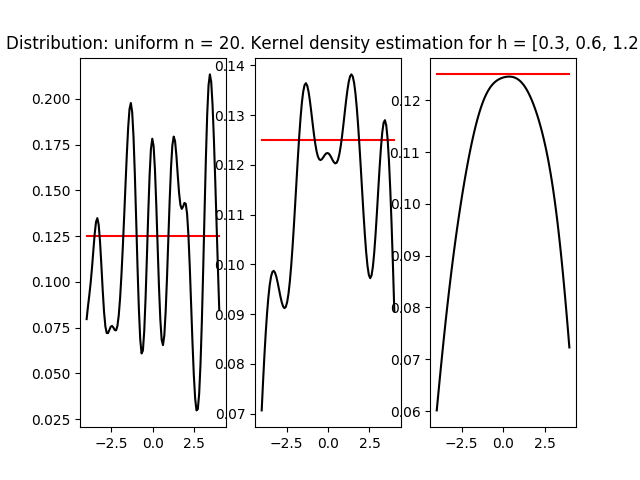
\includegraphics[width=\textwidth]{kernel/d_uniform20.png}
\end{figure}
    \begin{figure}[H]
 \caption{Ядерная функция плотности для равномерного распределения, n = 60}
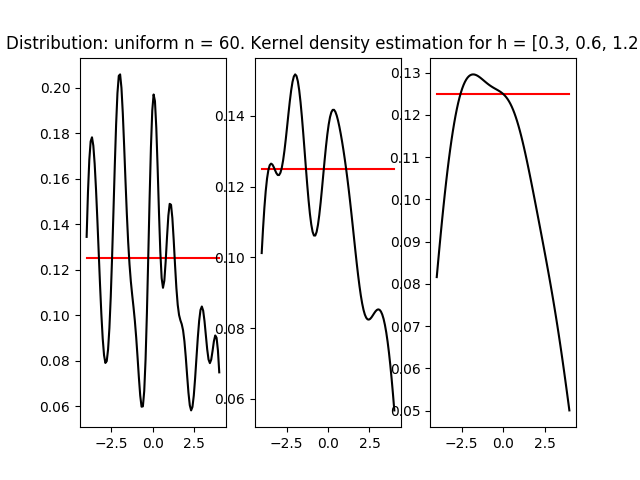
\includegraphics[width=\textwidth]{kernel/d_uniform60.png}
\end{figure}
    \begin{figure}[H]
 \caption{Ядерная функция плотности для равномерного распределения, n = 100}
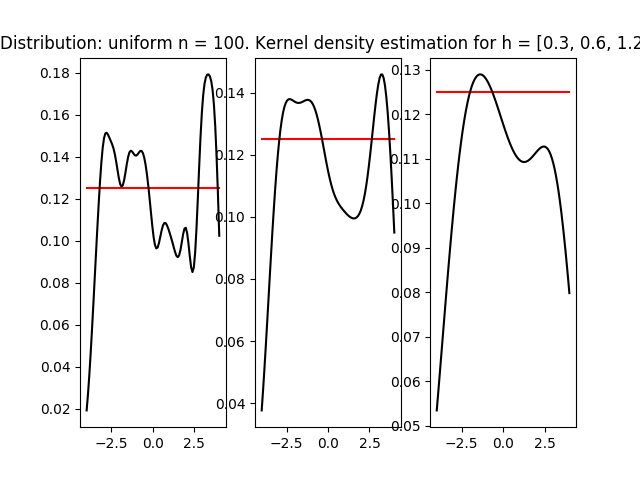
\includegraphics[width=\textwidth]{kernel/d_uniform100.png}
\end{figure}
\end{center}


\section{Выводы}
Эмпирическая функция лучше приближает эталонную функцию на больших выборках.

Наилучшее приближение функции распределения ядерной функции получено при наибольшей ширине окна. При фиксированной ширине окна точнее приблизить функцию распределения позволяет увеличение выборки.

\section{Приложения}

Исходники: \url{https://github.com/LanskovNV/math_statistics/tree/master/lab_4}

\newpage

%%%
% Literature
%%%
\begin{thebibliography}{}
    \bibitem{numpy}  Модуль numpy  -  https://physics.susu.ru/vorontsov/language/numpy.html
    
    \bibitem{average}  
    Выборочное среднее  -  https://en.wikipedia.org/wiki/Sample\_mean\_and\_covariance
    
    \bibitem{med}  
    Выборочная медиана  -  http://femto.com.ua/articles/part\_1/2194.html
    
    \bibitem{mean_extr}  
    Полусумма экстремальных значений  -  https://studopedia.info/8-56888.html
    
    \bibitem{quartiles}  
    Квартили  -  https://studfiles.net/preview/2438125/page:13/
    
    \bibitem{cut_mean}  Усечённое среднее  -  https://ole-olesko.livejournal.com/15773.html
\end{thebibliography}

\end{document}

